% Q1: Skin Depth and Electromagnetic Shielding
% Teaching diagram: shows wave attenuation through a material layer
\documentclass[border=10pt]{standalone}
\usepackage{tikz}
\usepackage{amsmath}
\usetikzlibrary{patterns, decorations.pathreplacing, arrows.meta}

\renewcommand{\familydefault}{\sfdefault}

\begin{document}
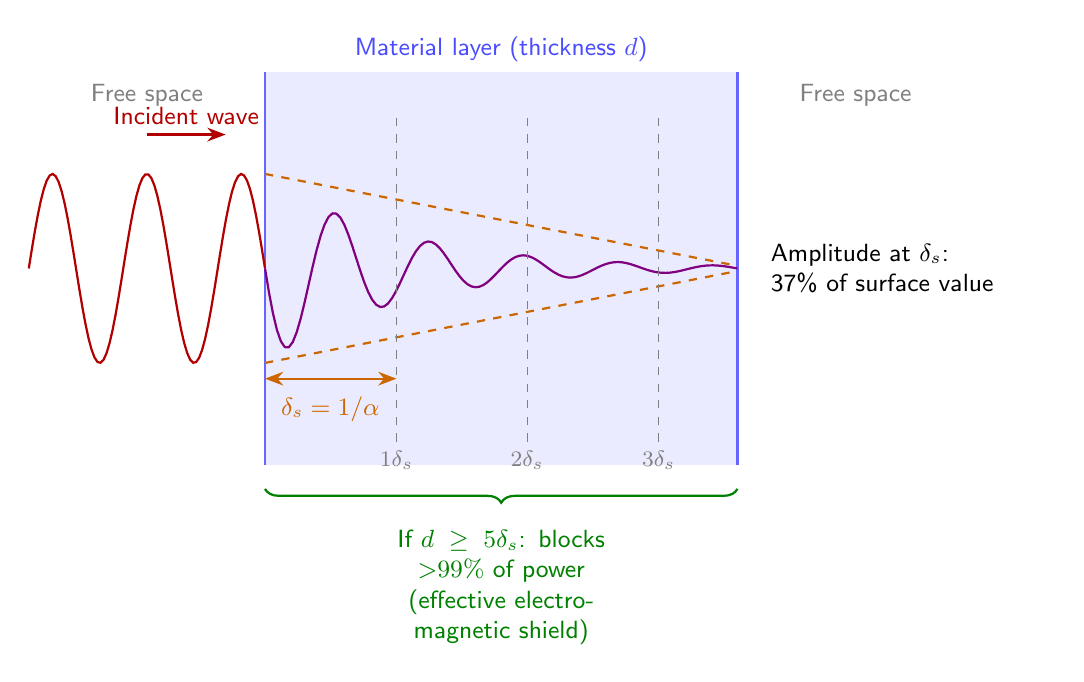
\begin{tikzpicture}[
    every node/.style={font=\sffamily\normalsize},
    >=Stealth
]

% --- Material slab ---
\fill[blue!8] (3,0) rectangle (9,5);
\draw[thick, blue!60] (3,0) -- (3,5);
\draw[thick, blue!60] (9,0) -- (9,5);
\node[above, blue!70, font=\sffamily\small] at (6,5) {Material layer (thickness $d$)};

% --- Region labels ---
\node[font=\sffamily\small, gray] at (1.5,4.7) {Free space};
\node[font=\sffamily\small, gray] at (10.5,4.7) {Free space};

% --- Incident wave (sinusoidal, constant amplitude) ---
\draw[thick, red!70!black, domain=0:3, samples=80]
    plot (\x, {2.5 + 1.2*sin(360*\x/1.2)});
\draw[->, thick, red!70!black] (1.5,4.2) -- (2.5,4.2)
    node[midway, above, font=\sffamily\small] {Incident wave};

% --- Exponential decay envelope inside material ---
\draw[thick, dashed, orange!80!black, domain=3:9, samples=2]
    plot (\x, {2.5 + 1.2*exp(-0.6*(\x-3))});
\draw[thick, dashed, orange!80!black, domain=3:9, samples=2]
    plot (\x, {2.5 - 1.2*exp(-0.6*(\x-3))});

% --- Decaying wave inside material ---
\draw[thick, red!50!blue, domain=3:9, samples=120]
    plot (\x, {2.5 + 1.2*exp(-0.6*(\x-3))*sin(360*(\x)/1.2)});

% --- Skin depth markers ---
\foreach \n/\xpos in {1/4.67, 2/6.33, 3/8.0} {
    \draw[thin, gray, dashed] (\xpos, 0.3) -- (\xpos, 4.5);
    \node[below, font=\sffamily\footnotesize, gray] at (\xpos, 0.3) {$\n\delta_s$};
}

% --- Amplitude annotations ---
\draw[<->, thick, orange!80!black] (3, 1.1) -- (4.67, 1.1);
\node[below, font=\sffamily\small, orange!80!black] at (3.83, 1.0) {$\delta_s = 1/\alpha$};
\node[right, font=\sffamily\small, text width=3.5cm] at (9.3, 2.5)
    {Amplitude at $\delta_s$:\\37\% of surface value};

% --- Teaching annotation: 5 skin depth rule ---
\draw[thick, green!50!black, decorate, decoration={brace, amplitude=5pt, mirror}]
    (3, -0.3) -- (9, -0.3);
\node[below, font=\sffamily\small, green!50!black, text width=4cm, align=center] at (6, -0.7)
    {If $d \geq 5\delta_s$: blocks ${>}99\%$ of power\\(effective electromagnetic shield)};


\end{tikzpicture}
\end{document}
